%---------------------------------------------------------------------
%
%                          Cap�tulo 3
%
%---------------------------------------------------------------------

\chapter{Review Study}

\begin{FraseCelebre}
\begin{Frase}
Work It Harder Make It Better\\
Do It Faster, Makes Us stronger\\
More Than Ever Hour After\\
Our Work Is Never Over 
\end{Frase}
\begin{Fuente}
Thomas \& Guy-Manuel, Daft Punk
\end{Fuente}
\end{FraseCelebre}

\begin{resumen}
A model for our cognitive node is defined in this chapter. Initially, the First Cognitive Device is evaluated
to obtain some guidelines and potential improvements facing our design. The final device implementation requirements and
constraints are defined. Finally, a discussion and evaluation over different modules is carried out, exposing different 
commercial options and concluding with some final decisions.
\end{resumen}

%-------------------------------------------------------------------
\section{Cognitive Wireless Sensor Network Node Model}
%-------------------------------------------------------------------
\label{cap3:sec:nodeModel}
%-------------------------------------------------------------------
Basically, the \ac{CWSN} node scheme responds to a standard \ac{WSN} model based on a microcontroller, radio and sensor interfaces, and power supply. However, a further review shows some general differences:

\begin{itemize}

\item \emph{Multiple Radio Interfacing}: Regarding \ac{CR} capabilities for spectrum management and \ac{DSA}, the node
	must include multiple \ac{RI}s enabling different spectrum bands instead of a single one. This capability
	is referred to the hardware modules. 

\item \emph{Multiple Control/Sensor Interfacing}: Since the device will serve as a standard \ac{CWSN} platform, it must
	embed different multi-purpose generic interfaces\footnote{These interfaces cover the usual peripherals and buses such as \ac{I2C}, \ac{SPI}, \ac{UART}, \ac{USB}, etc.}. This fact affects the hardware design of the device.

\item \emph{Protocol Stacking}: In order to enable communication over the different interfaces, the model must provide proper access to the lower layers of a communication protocol stack for each \ac{RI}\footnote{As it will be described, the employed firmware supposes a great software development since it maintains a single stack shared by all the interfaces.}. This affects the running firmware. 

\item \emph{Cognitive Layer}: Software implementations responsible to carry out all the cognition algorithms and computations. \ac{KP} and data flow management. Extra compute capabilities might be needed to give support to this layer. The already named \ac{CRMODULE} must carry out functions belonging to this domain.

\end{itemize}

\figura{Bitmap/Capitulo3/CWSNmodel}{width=.9\textwidth}{fig:CWSNnodeModel}%
{CWSN node model.}
%poner una unica pila

Figure \ref{fig:CWSNnodeModel} gives a view about the basic seeked model. It shows together software and hardware modules in a simplified way.
Additionally, cognition tasks compulsory require several functions to take into account at the design stage: 

\begin{itemize}

\item \emph{Power management}. Efficiency and low-power consumption are crucial following the inherent trend in \ac{WSN}s. Once deployed, it is common not having or barely having access to the nodes. Replacing batteries to an entire \ac{WSN} might become an infeasible task. The model should be able to include an autonomous power supply and other functions:

\begin{itemize}
\item \ac{TX} and \ac{RX} power regulation.
\item Unused modules disconnection.
\item Power-saving sleeping modes for transceivers and \ac{MCU}.
\end{itemize}

\item \emph{Spectrum management}. Some of the mainly needed functions:

\begin{itemize}
\item \ac{RSSI} detection.
\item Channel switching.
\item Energy scans all over the available frequencies range.
\end{itemize}

\end{itemize}

All the previous considerations give support to establish cognitive capabilities to the final application. These considerations, along with the requirements to be defined, will body the model of the final \ac{CNGD} implementation.

%-------------------------------------------------------------------
\section{First Cognitive Device review}
%-------------------------------------------------------------------
\label{cap3:sec:fcdEvaluation}
%-------------------------------------------------------------------

\figuraEx{Bitmap/Capitulo3/placaFer}{width=.8\textwidth}{fig:fcdnode}%
{Picture of the FCD, developed at LSI in 2011, obtained from \cite{juanpfc}.}{Picture of the FCD, developed at LSI in 2011.}

The \ac{FCD} was developed in 2011 at the \ac{LSI} by Fernando Lopez Lara \cite{ferpfc}. It supposed the first hardware platform fully oriented to \ac{CWSN} development that included three \ac{RI}s. Integrating hardware and software, it gave the chance to develop and test algorithms, strategies and applications for \ac{CWSN}. Moreover, it allowed to analyze suitability for radio interfaces, compute capability, and other components. It gave the strengths and weaknesses to establish the fundamentals for future designs. 

While constituting the first device meeting its features, the \ac{FCD} introduced several improvable issues found after its implementation and evaluation. Its power consumption, size and cost, together with other not achieved but desired requirement, make the device unsuitable for \ac{CWSN} test-bedding purposes and claim for a new design \cite{juanpfc}.

The \ac{FCD} has a Microchip \ac{PIC} hosting a \ac{MIPS} M4K, a 32-bits \ac{MCU} unit. It has a Harvard architecture employing a five-stages pipeline and a \ac{RISC}. The chosen model, a PIC32MX795F512H \cite{pic32datasheet}, integrates a 512 KB Flash Memory and a 128 KB general purpose \ac{SRAM}. It allows a maximum 80 MHz clock frequency and it achieves a throughput as high as 1.65 DMIPS/MHz\footnote{\ac{DMIPS} divided by \ac{CPU} frequency. Dhrystone is a synthetic computing benchmark program become representative of general processor performance.}.
This \ac{PIC} was found to offer too high features for our requirements, hence existing a reducible amount of power consumption 
on this module. Reducing capacity with regards to Flash and \ac{RAM} memory is seen as a positive option.  

The \ac{FCD} includes three \ac{RI}s enabling access to two different spectrum regions. Two of the selected interfaces
work on the 2.4 GHz band and the third one over the 868 MHz, corresponding to the \ac{ISM} bands in most part of Region 1. To operate over the 868 MHz band it used a Tulio$^{TM}$ \cite{tulio} transceiver oriented to \ac{LOWPAN} and IEEE 802.15.4
compatible. For the 2.4 GHz band, two Microchip modules were selected. A MRF24J40 \cite{mrf24j40} module using Microchip proprietary protocols such us MiWi$^{TM}$ P2P \cite{miwip2p}, MiWi$^{TM}$ Mesh, or MiWiPRO$^{TM}$ \cite{miwipro} and a MRF24WB0MA \cite{mrf24wb0} module, IEEE 802.11 compatible, as WiFi.
Firmware running on the \ac{FCD} operated by using three different protocol stacks. Tulio$^{TM}$ firmware was provided by \ac{AWD} and communications with the \ac{MCU} take place through an \ac{UART}. Stacks for MiWi \cite{miwi} and TCP/IP \cite{tcpip} protocols are provided freely by Microchip, being the first one significantly lighter and simpler than the second one. Communications with these transceivers use \ac{SPI} interfaces.

\figuraEx{Bitmap/Capitulo3/fcdmodel}{width=0.9\textwidth}{fig:fcdmodel}%
{Architecture model of the FCD, developed at LSI in 2011, obtained from \cite{juanpfc}.}{Architecture model of the FCD.}

The Tulio$^{TM}$ module offers a very low-consumption but it contains a Texas Instruments microcontroller increasing complexity on the global structure, moreover, this fact raises the global consumption up. Maintaining this interface will be disputed.
On the other hand, the WiFi interface seems to be inappropriate for \ac{WSN} due to its high power consumption, hibernation-related problems, and its complex, resources-consuming communication stack. Even though this interface is thought as a gateway, new options are highly needed. MRF24J40 gives a throughput suitable for the already described requirements, thus it could be a good candidate for the new design.

Regarding firmware options, the situation resulting from combining three different stacks becomes messy, confusing, power and resources-consuming, not suitable to deal properly with an application and a cognitive layer. Hence, using the developed \ac{HAL} \cite{juanpfc} that integrates three stacks and presents a straightforward \ac{API} for upper layers, seems a good choice for this work.

The node comprises two \ac{USB} terminals and an RS232 interface for debugging and interconnection purposes. Power supply system accepts 3.3 V and 5 V options including a voltage regulator and a charge pump.

Maintaining all these interfaces supposes larger device size and greater power consumption. A review about keeping all them as well as all the power supply options will be brought to pass, some of them seemed unuseful and inefficient.

Regarding other issues, reducing the general size, making the device more scalable or modular are indeed needed on the \ac{CNGD}.

%-------------------------------------------------------------------
\section{Firmware review}
%-------------------------------------------------------------------
\label{cap3:sec:halreview}
%-------------------------------------------------------------------

The work in \cite{juanpfc} described an implemented new firmware for the \ac{CNGD}. The firmware runs over PIC32 architectures. It was developed over the \ac{FCD} but slightly adapting the hardware for better performance\ref{guillepfc}. The firmware offers access to three different regions over the radio spectrum by means of Microchip transceivers and an appropriately modified and adapted MiWi$^{TM}$ protocol stack that allows using more than one PHY layer.

In order to abstract the application from the hardware and software complexity design, the firmware includes a straightforward \ac{HAL} to deal easily with the \ac{RI}s within a close set of functions. In this way, node usability improves and applications cost and developing time decrease.

The new firmware supposes several advantages:
	
\begin{itemize}

\item Versatility and adaptability are given. Hardware modifications and new modules are possible with minimal software adaptation.
\item Firmware takes care of the protocol stack management. 
\item MiWi$^{TM}$ protocol stack adaptation makes a better efficient use of resources and removes complexity.
\item Devices fabrication costs are reduced since some modules are not needed anymore and less featured controllers are suitable.
\item Sleeping modes provided by the firmware bring the key for autonomous operation modes. Whenever circumstances permit it, enabling sleeping modes will drop significantly the power consumption.
\end{itemize}

This software module must be taken into account at the design stage for its inclusion into the \ac{CNGD}. It also might be needed of adaptation or debugging tasks due to its short life-time and usage. 

%-------------------------------------------------------------------
\section{Cognitive Radio Module review}
%-------------------------------------------------------------------
\label{cap3:sec:crmodulereview}
%-------------------------------------------------------------------

This module is designed to operate under PIC32 architectures. It was thought to run over the previous described firmware. Its development took place over the \ac{FCD} and all the implementation proccess is set out on \cite{guillepfc}.

This software module represents an actual realization of the architecture described in \cite{conbrok} and, somewhat, enhances it by introducing sligth changes. 

An overview to the general performance shows an scheme based on different modules such as Repository, Discovery, Optimization, Execution, Access Control, Policy, Messenger and Virtual Control Channel. Each module performs a defined tasks and connect each other attending to defined policies. Figure \ref{fig:cap3:crmodel} illustrates the general scheme, for a further view consult the given references.

\begin{figure}[!h]
\centering
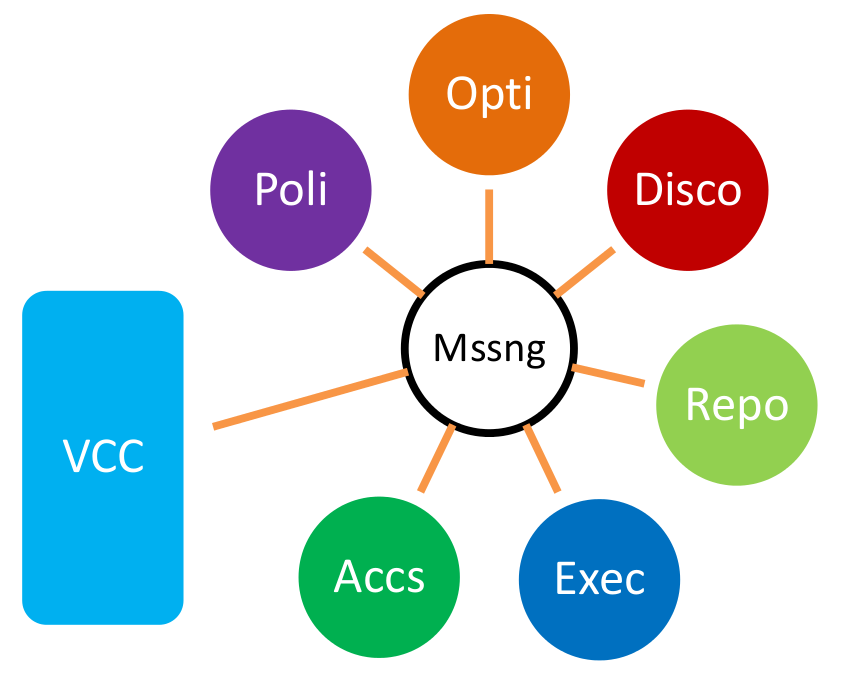
\includegraphics[width=0.6\textwidth]{Imagenes/Bitmap/Capitulo3/crmodule2}%
\caption[CRmodule architecture.]{CRmodule architecture, obtained from \cite{guillepfc}.}
\label{fig:cap3:crmodel}
\end{figure}

%-------------------------------------------------------------------
\section{System Requirements}
%-------------------------------------------------------------------
\label{cap3:sec:systemRequirements}
%-------------------------------------------------------------------

Once described the \ac{CWSN} node model and after evaluating the main related developments, it is time to define the requirements for the \ac{CNGD}. These are classified as follows:

\begin{itemize}

\item Essential requirements

\begin{itemize}

\item Communication possibilities, at least, over two \ac{ISM} bands (868 MHz and 2.4 GHz). Having, as far as possible, fully-configurable transceivers.
\item Modularity.
\item IEEE 802.11 standard inter-operation possibilities.
\item External pluggable antenna possibilities.
\item Development-oriented. Comprising debugging tools.
\item Working under a single development framework.
\item Useful and powered to try concepts referred to optimization strategies for:

\begin{itemize}
	\item Security.
	\item Power consumption.                   
	\item Synchronization.
	\item \ac{QOS}.
\end{itemize}

\end{itemize}
\item Desirable features
\begin{itemize}
  \item Portable and autonomous power supply options.
  \item Remote application-loader.
  \item Reduced size.
  \item Communication over three \ac{ISM} bands (433 MHz, 868 MHz, 2.4 GHz).
  \item Mono-core-based architecture.
  \item Battery charge-state monitoring.
  \item Real radio headers switching possibilities so as to use a single transceiver for more than one frequency band.
\end{itemize}
\end{itemize}

In addition, it should respond to standard requirements for \ac{WSN}s: 

\begin{itemize}

\item \emph{Scalability}. Given the potentially large amount of nodes composing a \ac{WSN}, the model claims for a easily scalable design.

\item  \emph{Cost}. Due to the same previous reason, low-cost is a requirement. Otherwise their price make networks unrealizable.

\item \emph{Ubiquitous computing}. Each node hosts some computing capacity, this gives to the network the chance for distributed cognition.
	Hence, robustness and stability is given to the set.

\item  \emph{Power consumption}. It must be prepared to  operate supplied by a battery and achieve a certain autonomy.

\item \emph{Throughput}. Performance must be high enough for a test-bed platform. Regarding the generic nature of the platform, it should be prepared for a wide range of applications. Cognition, on the other hand, increases as well the need for computation capabilities.

\item \emph{Communication data-rate}. Not too high data-rate transmissions are usually needed. Few tens or hundreds of kbps are enough.

\item \emph{Security}. Radio Interfaces allowing manageable security mechanisms. Being possible to safely deal with confidential or private data. 

\end{itemize}

%-------------------------------------------------------------------
\section{Technology}
%-------------------------------------------------------------------
\label{cap3:sec:technology}
%-------------------------------------------------------------------
Step by step, all the needed technologies for our design will be evaluated and compared to the employed by the \ac{FCD}.

%-------------------------------------------------------------------
\subsection{Microcontroller}
%-------------------------------------------------------------------
Based on the requirements described in \ref{cap3:sec:systemRequirements}, it seemed necessary to keep the number of cores reduced to one unit.
Furthermore, using a 32-bits Microchip \ac{PIC} was an imposed design decision, as it was said. 

The criteria to choose a microcontroller were:
\begin{itemize}
\item The less featured and simplest microcontroller that suits our operation memory parameters. \ac{FCD} showed that a Flash memory above 200 KB was enough and a \ac{RAM} memory over 32 KB fits our needs. This helps to keep down the microcontroller power consumption. All 32-bits \ac{PIC}s family posses a high enough throughput.

\item Some peripherals are essential to accomplish required tasks. At least three \ac{SPI}s\footnote{Most of commercial radio transceivers set
their communication with the \ac{MCU} over \ac{SPI}s} would be needed to interface the microcontroller and the radio transceivers. In addition, peripherals for debugging such as \ac{UART}s or \ac{USB}s must be simultaneously available. Apart from that, it should contain other buses and accessible peripherals for modularity. Probably a 100-pins microcontroller could provide better access to multiple peripherals than smaller sizes.

\item Lowest price.        
\end{itemize}

The different options included at Microchip catalog, described and showing their main features, are shown in table \ref{cap3:tab:micros}.

\begin{table}[h]
\centering
\scalebox{0.7}{
\begin{tabular}{||c | c | c | c | c | c | c | c | c | c | c | c | c | c ||}
\hline
\hline
\multicolumn{14}{|c|}{32-bits Microchip microcontrollers} \\
\hline
\multirow{2}{*}{Microcontroller} & \multirow{2}{2cm}{Max. \\Frequency} & \multicolumn{2}{c|}{Memory (KB)} & \multicolumn{6}{c|}{Peripherals} & \multirow{2}{*}{ADC} & \multirow{2}{*}{Pins} & \multirow{2}{*}{Consumption} & Price \\\cline{3-10}
& & Flash & RAM & SPI & UART & I2C & USB & CAN & ETH  & & & & (\euro)\\
\hline \hline
PIC32MX664F128H & \multirow{12}{*}{80} &  \multirow{4}{*}{128} & \multirow{4}{*}{32} & 3 & \multirow{12}{*}{6} & 4 & \multirow{12}{1cm}{Full Speed Host Dev. OTG} & \multirow{2}{*}{0} & \multirow{12}{1.1cm}{10/100 BaseT} & \multirow{12}{*}{16} & 64 & \multirow{4}{2.2cm}{Run: 39 mA   Idle: 17 mA  Sleep: 20 $\mu$A} & 5.80 \\
PIC32MX664F128L & & & & 4 && 5 &&&&& 100 && 6.41 \\\cline{1 - 1} \cline{5 - 5}\cline{7 - 7}\cline{9 - 9}\cline{12 - 12}\cline{14 - 14}
PIC32MX764F128H & & & & 3 && 4 && \multirow{2}{*}{1} &&& 64 && 5.95 \\
PIC32MX764F128L & & & & 4 && 5 &&&&& 100 && 6.54 \\\cline{1 - 1} \cline{3 - 5}\cline{7 - 7}\cline{9 - 9}\cline{12 - 12}\cline{13 - 14}
PIC32MX675F256H & & \multirow{4}{*}{256} & \multirow{6}{*}{64} & 3 && 4 && \multirow{2}{*}{0} &&& 64 &\multirow{6}{2.2cm}{ Run: 85 mA Idle: 36 mA  Sleep: 41 $\mu$A} & 7.11\\
PIC32MX675F256L & & & & 4 && 5 &&&&& 100 &&  8.35\\\cline{1 - 1} \cline{5 - 5}\cline{7 - 7}\cline{9 - 9}\cline{12 - 12}\cline{14 - 14}
PIC32MX775F256H & & & & 3 && 4 && \multirow{2}{*}{2} &&& 64 && 8.07\\
PIC32MX775F256L & & & & 4 && 5 &&&&& 100 && 8.79 \\\cline{1 - 1} \cline{3 - 3} \cline{5 - 5}\cline{7 - 7}\cline{9 - 9}\cline{12 - 12}\cline{14 - 14}
PIC32MX775F512H & & \multirow{4}{*}{512} & & 3 && 4 && \multirow{2}{*}{2}&&& 64 && 8.75 \\
PIC32MX775F512L & & & & 4 && 5 &&&&& 100 && 9.47 \\\cline{1 - 1} \cline{4 - 5}\cline{7 - 7}\cline{9 - 9}\cline{12 - 12}\cline{13 - 14}
PIC32MX795F256H & & &  \multirow{2}{*}{128} & 3 && 4 && \multirow{2}{*}{2} &&& 64 & Not & 9.47\\
PIC32MX795F256L & & & & 4 && 5 &&&&& 100 & Specified & 9.57\\
\hline
\hline

\end{tabular}
}
\caption{Comparative table of 32-bits family Microchip PICs.%
         \label{cap3:tab:micros}}
\end{table} 

%-------------------------------------------------------------------
\subsection{Radio Interfaces}
%-------------------------------------------------------------------
One of the desired requirements is enabling radio activity over three \ac{ISM} bands (434 MHz, 868 MHz and 2.4 GHz), so in order to achieve it, compatible transceivers on these bands must be studied. We first took two decisions based on the experience brought by the \ac{FCD}.

The \ac{FCD} access the 868 MHz band using a Tulio$^{TM}$ module. This module brings global complexity to the design, it includes a core itself and the communication between cores are driven by the \ac{UART}, the low data-rate communication provided does not seem to support our goals either. To keep the single-core architecture, lowering-down power consumption and meeting the described requirements, this module will be suppressed and it will be looked for a replacement.

MRF24WB0MA WiFi transceiver, embedded by the \ac{FCD}, raises up the power consumption to unsuitable levels in a \ac{WSN}. The protocol stack is very computationally heavy and memory-consuming compared other usual protocol stacks in \ac{WSN}s. New ways to establish a IEEE 802.11 gateway will be studied, maybe through a pluggable expansion module. The low-consumption, low-resources and simple scheme seeked in the \ac{CNGD} cannot afford to include this transceiver.

Table \ref{tab:cap3:ri} shows transceivers and modules supported by the chosen firmware that enables communication at the desired bands. Modules such as the MRF49XA PICtail$^{TM}$ Daughter Board, Figure \ref{fig:cap3:pictail}, whose size does not suit our requirements, have not been considered.

\begin{table}[h]
\centering
\scalebox{0.7}{

\begin{tabular}{||c|c|c|c|c|c|c|c|c|c||}
\hline
\hline
\multirow{2}{*}{Model} & Freq. & Compliant & Data Rate & Sensing & \multicolumn{4}{c|}{Consumption} & Price \\ \cline{6-9}
& (MHz) & Technologies & (kbps) & options & Tx & Rx & Sleep & Idle & (\euro) \\ \hline \hline

MRF49XA & 434/ & \multirow{6}{*}{MiWi$^{TM}$} &\multirow{2}{*}{250} & \multirow{6}{*}{RSSI} & I433=26 mA @ 7 dBm  & I433=13 mA. & \multirow{2}{*}{0.3 $\mu$A} & \multirow{2}{*}{1.2 mA} & \multirow{2}{*}{2.84} \\
(transceiver) & 868/915 & & & & I868=27 mA @ 5 dBm  & I868=14 mA & & & \\  \cline{1-2} \cline{4-4} \cline{6-10}
MRF89XA & 868/ & & \multirow{2}{*}{200} & & & \multirow{4}{*}{3.5 mA} & \multirow{4}{*}{0.1 $\mu$A} & \multirow{4}{*}{60 $\mu$A} &\multirow{2}{*}{3.86} \\ 
(transceiver) & 915/955 & & & & 25 mA @ +10 dBm  & & & & \\ \cline{1-2} \cline{4-4} \cline{10-10}
MRF89XAM8A & \multirow{2}{*}{868} & & FSK: 40 & & 16 mA  @ +1 dBm &  & & & \multirow{2}{*}{8.26} \\ 
(module) & & & OOK: 16 & &   & & & & \\ \hline \hline
\end{tabular}}

\caption{Comparative table of sub-GHz Microchip solutions\label{tab:cap3:ri}}

\end{table}

\figura{Bitmap/Capitulo4/pictail}{width=.4\textwidth}{fig:cap3:pictail}%
{MRF49XA PICtail$^{TM}$ Daughter Board}

There are not complete modules available for 434 MHz band. For 868 MHz, module MRF89XAM8A is available. However, MRF49XA transceiver, which provies communications at these two bands, is susceptible to be included into an ad-hoc designed \ac{RI} board. Figure \ref{fig:cap2:wirelesscomparison} gives a comparison among wireless networking protocols.

\figura{Bitmap/Capitulo3/wirelesscomparison}{width=.7\textwidth}{fig:cap2:wirelesscomparison}%
{Main wireless networking options comparison}

%-------------------------------------------------------------------
\subsection{Serial Communication}
%-------------------------------------------------------------------
Serial communication is a very important feature for applications development and debugging. It allows wiring the node and establishing communication between the \ac{CNGD} and any other device, normally a computer or storing devices to track data. Peripherals such as the \ac{UART} is commonly used to stablish these communication tasks. More recent implementations enable communications through \ac{USB}.

While the \ac{FCD} includes two \ac{USB} connectors, a $\mu$USB and normal one, together with an RS232 communication module, three communication ways to interface the node seems too many. These modules are size and power consuming.

$\mu$USB connectors show a reduced size compared to first connectors and they do expand the first connectors capabilities.

The idea of including a normal connector gives some interconnection opportunities with attachable devices like mouses, keyboards, or portable memories in which the node adopts a \emph{master} role facing a \emph{slave} device. This feature supposes the inclusion of a power consuming circuitry to raise the voltage up to 5 V into the USB, subtracting simplicity to the design. In order to fit the requirements, it does not seem to be needed this last capability on each node. A $\mu$USB connector would be enough.

RS232 communication so does needs its own power supply. The size and cost for an RS232 connector and circuitry, which requires a MAX3232 chip, is too high for a default serial communication module within each node. An optional module for RS232 might be a good option given its wide acceptance and utility in embbeded systems despite the global use of \ac{USB}.

%-------------------------------------------------------------------
\subsection{Power Supply System}
%-------------------------------------------------------------------
The power supply system designed for the \ac{FCD} includes some modules susceptible to be suppressed or replaced to keep the simplicity and
reduce the consumption. 

The MCP1612 \cite{mcp1612} buck regulator specifications fit the supply requirements on excess, so a less-featured component might be enough at the new design. The maximum output current for the MCP1612, up to 1 A, could be significantly reduced. 

The MCP1253-33X \cite{mcp1252} charge-pump, responsible for raising the voltage up to 5V to operate over \ac{USB} as master, could be removed in the new design if this option is not finally implemented.

%-------------------------------------------------------------------
\subsection{Timing}
%-------------------------------------------------------------------
Timing options included on the \ac{FCD} suppose a low-consumption oscillator for real-timing and a second oscillator for maximum operation frequency. 
It does not appear any problem related to the timing configuration. The defined configuration fits the requirements and, firstly, seems a good
option to keep it unchanged.

%-------------------------------------------------------------------
\subsection{Application Capabilities}
%-------------------------------------------------------------------
Application capabilities over the \ac{FCD} are poor. Apart from interacting with the \ac{RI} and serial communication, the board does not offer
options for sensing/controlling applications neither other more complex possibilities such as including new communication modules. 
This is because the \ac{FCD} does not embed any expansion header or slot where adapting any new design to expand to new features.

The new design calls for expansion options where application capabilities could be widely and easily opened by attaching modules including an ad-hoc design. A complete expansion header for a \ac{WSN} node should include access to the following peripherals/buses:

\begin{itemize}
\item \emph{\ac{I2C}}. Being the most common bus to interface sensors to the \ac{MCU}. 
\item \emph{\ac{USB}}. For serial communication, mainly with a host device.
\item \emph{\ac{UART}}. For asynchronous serial communication with devices.
\item \emph{\ac{SPI}}. As a usual serial communication peripheral.
\item \emph{Ethernet}. For IEEE 802.11 compatibility.
\item \emph{Interruptions}. Enabling interrupting the \ac{MCU} without employing polling.
\end{itemize}    

%-------------------------------------------------------------------
\section{Conclusions}
%-------------------------------------------------------------------
\label{cap3:sec:conclusions}
%-------------------------------------------------------------------
After having a review all over the, hardware and software, recent implementations related to \ac{CWSN}s that might bring some guidances in our design; after evaluating the used technology and analyzing the weaknesses; after defining some minimal requirements to fit, and applying them to our evaluations, the obtained conclusions to face the design stage follow:

\begin{itemize}
\item The model implemented by the \ac{FCD} is quite close to the one pursued. It will serve as guide in our designing process since its
	review reveals significant technology and behavioral-related information.

\item A new configuration regarding size and cost, allowing flexibility and modularity.

\item Implemented software such as the described firmware will help us saving time on the software development and it proposes a very complete solution that fits our requirements. It provides a shared protocol stack and a very useful \ac{HAL}. Even if needed some slight adaptations,
	it must be compatible with our \ac{CNGD} design.

\item \ac{FCD} includes a too featured microcontroller for our requirements, implying higher power consumption and cost. A new \ac{MCU}
	seems needed.
\item \ac{RI}s used by the \ac{FCD} open communication on two frequency bands. They show a very inefficient performance and high consumption behavior due to:
	\begin{itemize}
	\item Coexistence of three heterogeneous transceivers and different protocol stacks. Bringing complexity and operation inefficiency.
	\item Presence of a WiFi transceiver, with consumptions up 160mA at \ac{TX}.
	\item A Tulio$^{TM}$ transceiver whose inclusion, hosting a core by itself, supposes a multi-core implementation.  	
	\end{itemize}

A reconfiguration of the \ac{RI}s is needed. Bringing homogeneity and a \ac{WSN} standard protocol such as IEEE 802.15.4. In addition, desirable requirements call for a third frequency band to implement. The lack of fittable modules over 434 MHz band claims for a custom \ac{RI} design.

\item Serial communication system claims for simplifications, the same as the power supply system.

\item Application capabilities must be expanded to enhance modularity and node capabilities. Expansion pluggable options must access the main 		peripherals. Enabling the 802.11 standard is a requirement.

\item A portable supply system must urgently be completely developed.

\end{itemize}
%-------------------------------------------------------------------
%\section*{\NotasBibliograficas}
%-------------------------------------------------------------------
%\TocNotasBibliograficas
%Citamos algo para que aparezca en la bibliograf�a\ldots
%\citep{ldesc2e}

%\medskip

%Y tambi�n ponemos el acr�nimo \ac{CVS} para que no cruja.

%Ten en cuenta que si no quieres acr�nimos (o no quieres que te falle la compilaci�n en ``release'' mientras no tengas ninguno) basta con que no definas la constante \verb+\acronimosEnRelease+ (en \texttt{config.tex}).


%-------------------------------------------------------------------
%\section*{\ProximoCapitulo}
%-------------------------------------------------------------------
%\TocProximoCapitulo

%...

% Variable local para emacs, para  que encuentre el fichero maestro de
% compilaci�n y funcionen mejor algunas teclas r�pidas de AucTeX
%%%
%%% Local Variables:
%%% mode: latex
%%% TeX-master: "../Tesis.tex"
%%% End:
